% 11.
\section{}

% 11.a.
\subsection{}
Solve for $x_2$.
\begin{align*}
    Wx + b &= 0 \\
    \begin{bmatrix}
	-1 & 2 \\
    \end{bmatrix}
    \begin{bmatrix}
	x_1 \\
	x_2
    \end{bmatrix}
    + 2 
    &= 0 \\
    -x_1 + 2x_2 + 2 &= 0 \\
    -x_1 + 2x_2 &= -2 \\
    2x_2 &= x_1 - 2 \\
    x_2 &= \frac{1}{2}x_1 - 1  
\end{align*}

Plot the hyperplane. \\
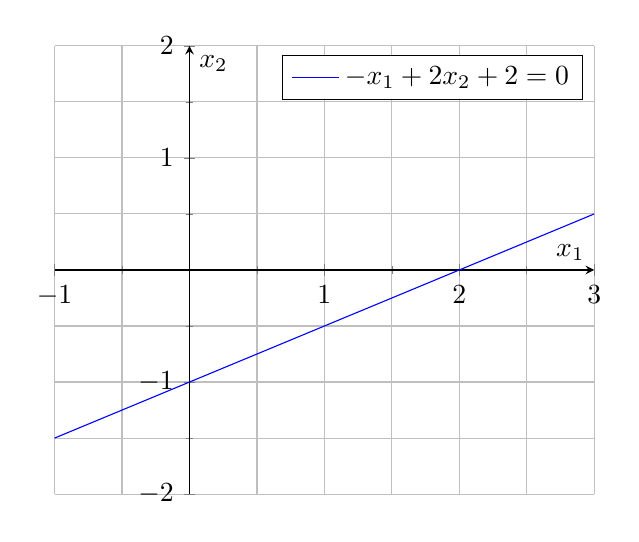
\begin{tikzpicture}
    \begin{axis}[
	grid=both,
	ymin=-2,
	ymax=2,
	xmin=-1,
	xmax=3,
	minor tick num=1,
	axis lines=middle,
	xlabel=$x_1$,
	ylabel=$x_2$
    ]
    \addplot [
	samples=100,
	color=blue
	]	
	{1/2*x - 1};
    \addlegendentry{$-x_1 + 2x_2 + 2 = 0$}
    \end{axis}
\end{tikzpicture}

% 11.b.
\subsection{}

Solve for $x_3$.
\begin{align*}
    Wx + b &= 0 \\
    \begin{bmatrix}
	1 & 1 & 1
    \end{bmatrix}
    \begin{bmatrix}
	x_1 \\
	x_2 \\
	x_3
    \end{bmatrix}
    + 0
    &= 0 \\
    x_1 + x_2 + x_3 &= 0 \\
    x_3 = -x_1 - x_2 \\ 
\end{align*}

Plot the hyperplane. \\
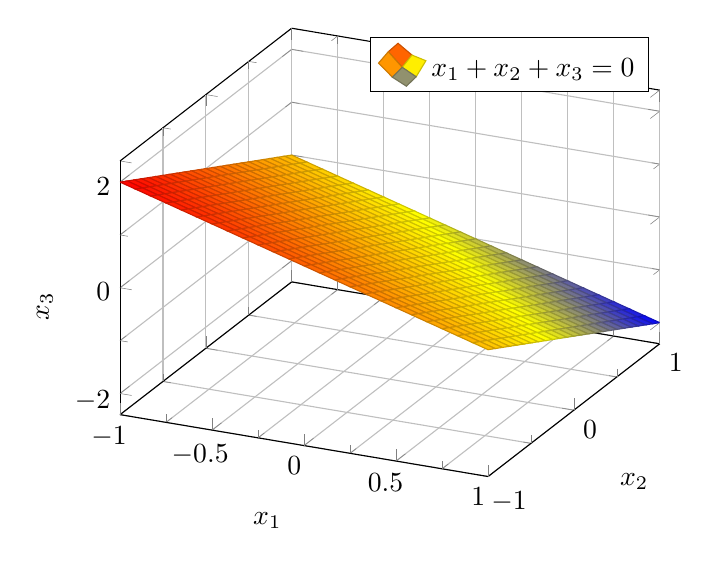
\begin{tikzpicture}
  \begin{axis}[
	grid=both,
	domain=-1:1,
	y domain=-1:1,
	minor tick num=1,
	xlabel=$x_1$,
	ylabel=$x_2$,
	zlabel=$x_3$
    ]
    \addplot3[surf] {-x -y};
    \addlegendentry{$x_1 + x_2 + x_3 = 0$}
  \end{axis}
\end{tikzpicture}

% 11.c.
\subsection{}

Find $\min_{x} ||x_0 - x||^2$ such that $w^T x + b = 0$. Let $\tilde{x}_0$ be the minimizer to the problem.  
\begin{align*}
    ||x_0 - \tilde{x}_0|| &= |\frac{w^T (x_0 - \tilde{x}_0)}{||w||}| \\
    ||x_0 - \tilde{x}_0||^2 &= |\frac{w^T (x_0 - \tilde{x}_0)}{||w||}|^2 \\ 
    &= |\frac{w^T x_0 + b}{||w||}|^2
\end{align*}

